\chapter{프리드만 동역학과 상태방정식}

\lectureoverview{균일 팽창은 국소적으로 속박된 물리 현상과 구분해야 하며, 내재적 기하학은 매장된 모양과 구분해야 한다. 이러한 구분이 명확해지면 우주론적 원리에 따라 시공간 계량은 하나의 척도 인자 \(a(t)\)와 하나의 곡률 표지 \(k\)로 정해진다. 아인슈타인 방정식의 시간-시간 성분은 프리드만 에너지 방정식이 된다. 이 방정식을 풀려면 압력과 에너지 밀도 사이의 물질 관계가 더 필요하다. 단열 열역학과 상태방정식 \(P=w\rho\)은 \(\rho\propto a^{-3(1+w)}\)을 주어 물질, 복사, 진공 에너지를 하나의 틀로 통합한다.}

\section{물리적 그림을 정립하는 질문들}

\subsection{지평선보다 앞서 공간이 반복될 수 있을까?}

유한한 평탄 우주는 주기적인 셀로 나타낼 수 있다. 그 셀이 관측 가능한 영역보다 작다면 빛은 셀을 가로질러 이동할 수 있고, 하늘에는 같은 구조를 반복해서 본 모습이 나타날 것이다. 이러한 반복을 찾아내는 일은 익숙한 은하를 알아보는 것보다 어렵다. 영상은 서로 다른 방향과 시기에 도달하며, 우주의 진화에 따라 달라지기 때문이다. 그럼에도 주기적 위상은 관측 가능한 결과를 낳는다.

\begin{classroomqa}
\audiencequestion{우주 전체가 관측 가능한 우주보다 작을 수 있을까요?}
\lecturerresponse{주기적으로 동일시된 토러스가 자연스러운 제안이다. 그렇다면 우리는 같은 물리적 영역의 반복된 복사본을 관측하게 되며, 비유적으로는 뒷문을 통해 우리 자신을 보는 셈이다. 이에 해당하는 우주 주기성을 찾으려는 조사에서 이를 뒷받침하는 증거는 나오지 않았으며, 작은 기본 셀의 크기에 제약을 두고 있다. 이 가능성은 기하학적으로 모순되지 않지만, 이미 관측한 영역보다 우주가 작다는 가설은 이 증거로 볼 때 지지받지 못한다. \lecturetimestamp{00:01:17--00:02:33}}
\end{classroomqa}

\subsection{팽창이 속박된 계를 벌려 놓지는 않는다}

우주 팽창은 평균적인 우주 기하에서 자유롭게 움직이는 물질의 대규모 운동을 나타낸다. 모든 고유 길이가 반드시 증가해야 한다는 보편적 명령은 아니다. 전자기력은 원자를 속박하고, 중력은 행성계를 속박하며, 분자간력은 고체를 속박한다. 이러한 상호작용은 해당 규모에서 우주론적 보정보다 압도적으로 강하다.

\begin{classroomqa}
\audiencequestion{팽창은 암흑 에너지 때문에 일어나나요? 원자나 행성 궤도는 왜 공간과 함께 팽창하지 않나요?}
\lecturerresponse{암흑 에너지가 발견되기 전부터 우주의 팽창은 알려져 있었다. 암흑 에너지는 팽창을 가속해 팽창 양상을 바꾸지만, 팽창의 정의도 최초 원인도 아니다. 속박된 계는 국소적인 힘이 우세하므로 허블 흐름을 따르지 않는다. 가속하는 배경은 원자나 궤도에 극히 작은 섭동을 일으킬 수 있지만, 보통의 속박력은 계가 흩어지게 두지 않고 거의 변하지 않는 평형 상태로 되돌린다. \lecturetimestamp{00:02:36--00:06:50}}
\end{classroomqa}

\subsection{시간에 따라 변하는 기하에서의 에너지}

남은 의문은 힘이 아니라 에너지 수지에 관한 것이다. 속박된 궤도가 작은 우주론적 섭동에 계속 저항한다면, 필요한 에너지는 어디서 오는가? 이 질문의 전제는 전역적인 시간 병진 대칭이 없는 시공간에 정적인 배경의 보존 법칙을 가져온다.

\begin{classroomqa}
\audiencequestion{국소적인 속박력이 팽창에 저항할 때 에너지는 어디서 오나요?}
\lecturerresponse{정적인 세계에서 에너지 보존이 성립하는 것은 시간 병진 대칭성 때문이다. 배경과 그 법칙은 실험을 시간상 이동해도 동일하게 보인다. 팽창하는 시공간은 그러한 전역적 의미에서 시간 병진 대칭적이지 않으므로, 우주 전체에 대해 하나의 보존되는 총에너지가 존재할 필요는 없다. 국소적인 응력-에너지 보존은 여전히 성립하며, 아래에서 연속 방정식으로 나타난다. 성립하지 않는 것은 기하가 변하는 동안 전역적으로 정의된 우주 에너지가 반드시 일정해야 한다는 순진한 주장이다. \lecturetimestamp{00:06:52--00:09:24}}
\end{classroomqa}

\subsection{균질성은 거친 규모에서 성립하는 진술이다}

우주론적 원리는 규모에 따라 달라진다. 닫힌 방 안의 공기는 방 크기에서는 거의 균일할 수 있지만 분자 규모에서는 알갱이 구조를 갖는다. 우주에도 행성, 은하, 은하단, 밀도 요동이 있다. 균질성과 등방성은 이러한 구조가 위치나 방향을 특별하게 만들지 않을 만큼 충분히 큰 거리에서 평균한 거동을 가리킨다.

\begin{classroomqa}
\audiencequestion{작은 규모의 속박 구조는 균질성과 등방성에 어긋나나요?}
\lecturerresponse{아니다. 개별 분자를 분해해 보면 공기가 균질하지 않은 것처럼, 작은 규모에서는 정확한 균질성이 성립하지 않는다. 수억 광년 이상의 규모에서 관측된 분포는 대략 균일하고 방향에 무관하다. 우리가 관측할 수 있는 영역 너머에서도 균질하다는 것은 확립된 사실이 아니라, 그 결과를 검증해야 하는 가정이다. \lecturetimestamp{00:09:27--00:10:55}}
\end{classroomqa}

\section{기하학적 진술로서의 균질성과 등방성}

균질성과 등방성은 동역학적 진술이 되기 전에 먼저 기하학적 진술이다. 아인슈타인 방정식은 기하가 시간에 따라 어떻게 변하는지 알려준다. 먼저 임의의 한 시점에서 어떤 공간 기하가 허용되는지 정해야 한다.

\begin{classroomqa}
\audiencequestion{균질성과 등방성은 수학적으로 무엇을 뜻하나요?}
\lecturerresponse{계량으로 공간을 기술하고 한 점을 원점으로 하는 좌표 \(x^i\)를 택하자. 이제 다른 점을 원점으로 하는 좌표 \(y^i\)를 택하자. 균질성이란 원점을 옮기는 변환을 해도 계량의 함수 형태가 그대로인 것을 뜻한다. 그러면 모든 점은 기하학적으로 서로 동등하다. 등방성은 각 점을 중심으로 한 회전 대칭을 더하여, 선호되는 방향이 없도록 한다. \lecturetimestamp{00:11:13--00:14:26}}
\end{classroomqa}

\begin{definition}
어떤 공간이 임의의 한 점을 다른 임의의 점으로 옮기는 등거리변환을 허용하면 \emph{균질}하다고 한다. 한 점을 중심으로 회전해도 기하가 변하지 않으면 그 점에서 \emph{등방}하다고 한다. 균질하면서 등방적인 공간에는 선호되는 위치도 방향도 없다.
\end{definition}

유클리드 평면은 이 정의를 명확하게 보여준다. 데카르트 좌표에서 계량은
\begin{equation}
ds^2=dx_1^2+dx_2^2.
\label{eq:c04-flat-metric}
\end{equation}
원점을 상수 \(a_1\)와 \(a_2\)만큼 옮기자:
\begin{equation}
y_1=x_1+a_1,
\qquad
y_2=x_2+a_2.
\label{eq:c04-flat-translation}
\end{equation}
\(dy_i=dx_i\)이므로, 평행이동된 계량은 다음과 같다.
\begin{equation}
ds^2=dy_1^2+dy_2^2.
\end{equation}
점의 위치를 표시하는 기호는 바뀌었지만 거리의 규칙은 바뀌지 않았다. 이것이 균질성을 가장 간단히 구현한 예다. 회전도 계량을 보존하므로 평면은 등방적이기도 하다.

구면은 좌표가 덜 편리하다는 점에서만 더 까다롭다. 남극을 원점으로 택하면 단위 2-구면은 다음과 같이 쓸 수 있다.
\begin{equation}
d\Omega_2^2=dr^2+\sin^2 r\,d\theta^2.
\label{eq:c04-sphere-metric}
\end{equation}
구면을 회전해 동극이 새 원점이 되게 하자. 좌표 변환은 복잡하지만, 결과는 다시 방정식~\eqref{eq:c04-sphere-metric}이다. 둥근 구면에는 기하학적으로 특별한 점이 없다.

\begin{classroomqa}
\audiencequestion{주기적으로 동일시된 평탄 토러스는 균질하면서 등방적인가요?}
\lecturerresponse{평행이동에 대해서는 균질하다. 주기 셀의 모든 점에서 국소 기하가 같기 때문이다. 하지만 동일시가 선호되는 주기 방향과 길이를 정하므로 완전한 등방성은 아니다. 그 축 중 하나를 따라 보는 것은 일반적인 비스듬한 방향을 보는 것과 전역적으로 다르다. 따라서 토러스는 완전한 등방성 없이 균질성만 갖는 명확한 예다. \lecturetimestamp{00:20:18--00:21:30}}
\end{classroomqa}

관측된 대규모 균일성은 우리의 지평선 안에서 우주론적 원리를 채택할 근거가 된다. 관측 가능한 영역 너머까지 이를 확장하는 것은 직접 관측이 아니라 가정이다. 이 가정을 받아들이는 이유는 자료와 대조할 수 있는 결과를 내는, 명확히 규정된 기하를 제공하기 때문이다.

\section{내재적 기하와 매장}

공간이 구형이라고 할 때 더 큰 방 안에 둔 풍선의 고무 표면을 떠올리기 쉽다. 이 그림은 시각화에 도움이 될 수 있지만, 주변의 방은 우주론적 주장의 일부가 아니다. 중요한 것은 \emph{내재적} 기하이다. 이는 공간 안에 머무는 관측자가 측정할 수 있는 거리와 각도로 이루어진다.

\subsection{닫힌 1차원 세계}

닫힌 1차원 세계를 생각해 보자. 이것을 원, 모서리가 둥근 정사각형, 또는 땅콩 모양의 고리로 그릴 수 있다. 선 위에 갇혀 사는 존재는 선을 따라 잰 거리만 측정할 수 있다. 두 고리의 전체 둘레가 같다면, 그림이 전혀 다르게 보여도 그 안의 존재가 경험하는 내재적 기하는 같다.

\begin{figure}[htbp]
\centering
\includegraphics[width=0.72\textwidth]{lecture_04_figure_05.png}
\caption{내재적 기하와 매장된 모양을 구분하기 위한 원형 고리와 변형된 고리. 이 후반 프레임에는 앞선 논의 중 그린 그림이 담겨 있으며, 관련 내용은 00:23:21--00:25:59에 나온다.}
\label{fig:c04-intrinsic-board}
\lectureframe{00:59:54.899}
\end{figure}

모든 1차원 계량은 국소적으로 평탄하다. 짧은 끈 조각은 늘이지 않고 곧게 펼 수 있으므로, 주변 평면에서 눈에 보이는 굽음은 내재적 곡률이 아니라 외재적 굽음이다. 닫힌 고리는 둘레라는 전역적 모듈러스를 갖지만, 그 1차원 세계 안의 거주자가 측정할 수 있는 내재적인 국소 굽음은 없다.

\begin{figure}[htbp]
\centering
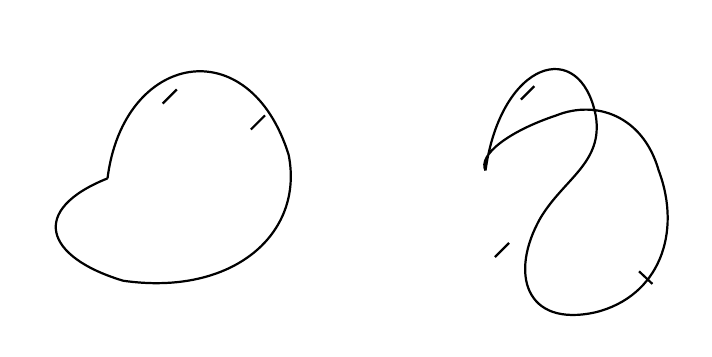
\begin{tikzpicture}[scale=1.0]
\draw[line width=0.8pt] (0,0)
  .. controls (0.2,1.6) and (1.8,1.9) .. (2.3,0.3)
  .. controls (2.5,-0.7) and (1.6,-1.5) .. (0.2,-1.3)
  .. controls (-0.8,-1.0) and (-1.0,-0.4) .. (0,0);
\draw[line width=0.8pt] (0.70,0.95) -- (0.88,1.13);
\draw[line width=0.8pt] (1.82,0.62) -- (2.00,0.80);

\draw[line width=0.8pt] (4.8,0.1)
  .. controls (5.0,1.5) and (6.0,1.8) .. (6.2,0.8)
  .. controls (6.3,0.2) and (5.8,0.0) .. (5.5,-0.5)
  .. controls (5.1,-1.2) and (5.3,-1.9) .. (6.2,-1.7)
  .. controls (7.0,-1.5) and (7.3,-0.7) .. (7.0,0.1)
  .. controls (6.8,0.8) and (6.2,1.0) .. (5.7,0.8)
  .. controls (5.1,0.6) and (4.7,0.3) .. (4.8,0.1);
\draw[line width=0.8pt] (5.25,1.00) -- (5.42,1.17);
\draw[line width=0.8pt] (5.10,-0.82) -- (4.92,-1.00);
\draw[line width=0.8pt] (6.75,-1.18) -- (6.92,-1.34);
\end{tikzpicture}
\caption{원을 다시 그린 그림과 변형된 고리. 둘레가 같으면 내재적인 1차원 기하도 같다.}
\label{fig:c04-intrinsic-redraw}
\end{figure}

\begin{classroomqa}
\audiencequestion{유한한 선분도 같은 종류의 1차원 공간인가요?}
\lecturerresponse{아니다. 선분에는 양 끝점이 있지만 닫힌 고리에는 끝점이 없다. 이 위상적 차이는 내재적이며, 두 물체 중 어느 하나를 더 큰 공간 안에서 구부려도 없앨 수 없다. 위상을 정하고 나면 선분은 길이로, 닫힌 고리는 둘레로 특징지어진다. \lecturetimestamp{00:26:00--00:26:39}}
\end{classroomqa}

\subsection{매장은 유용하지만 필수는 아니다}

1차원 원을 2차원 공간 안에 놓고 2차원 구면을 3차원 공간 안에 놓아 시각화한다. 이런 방식에 익숙해지면 3-구면을 논하기 전에 4차원 유클리드 공간이 필요하다고 생각하기 쉽다. 그러나 이는 인간의 시각화 능력에서 비롯된 요구이지 수학적 필연성은 아니다. 우리의 시각 능력은 3차원 공간에서 길을 찾도록 진화했다. 좌표와 계량을 이용하면 외부의 관점을 실제로 구성하지 않고도 그 한계를 넘어 추론할 수 있다.

\begin{classroomqa}
\audiencequestion{추가 공간 차원이 존재하지만 너무 작아 보이지 않을 수도 있나요?}
\lecturerresponse{그렇다. 기하학은 모든 차원이 관측 가능한 범위에서 같은 크기일 것을 요구하지 않는다. 콤팩트한 차원은 일상 경험이 탐사하는 규모보다 훨씬 작을 수 있다. 하지만 여기서 당장 중요한 점은 더 간단하다. 추가 차원이 물리적으로 존재하든 아니든, 우리 3차원 공간의 내재적 계량을 정의하는 데 매장 차원은 필요하지 않다. \lecturetimestamp{00:29:55--00:30:12}}
\end{classroomqa}

\begin{classroomqa}
\audiencequestion{굽은 선에 갇힌 존재는 선이 휘었는지 어떻게 알 수 있을까요?}
\lecturerresponse{내재적 측정만으로는 알 수 없다. 빛과 물질이 광섬유 안에 갇혀 있다고 생각해 보자. 광섬유를 늘이지 않고 구부려도 매장은 바뀌지만, 광섬유를 따라 측정한 거리나 신호 이동 시간은 바뀌지 않는다. 신호가 주변 공간으로 빠져나갈 수 있어야만 외부에서 휘어진 정도를 알아낼 수 있다. \lecturetimestamp{00:30:15--00:31:14}}
\end{classroomqa}

이 사고 실험은 실제 작동 방식으로 구체화할 수 있다. 광섬유에 갇힌 생명체가 충분한 에너지를 가진 광자와 같은 신호를 보낸다고 하자. 신호가 광섬유를 빠져나왔다가 1차원 계량 안에서는 불가능한 경로를 따라 돌아오는 경우에만 외부 방향을 알아낼 수 있다. 같은 맥락에서, 보통의 공간에 큰 차원이 3개 있다는 진술은 인간이 상상할 수 있는 것으로부터의 연역이 아니라 궁극적으로 실험에 근거한다.

\begin{classroomqa}
\audiencequestion{모든 1차원 공간이 국소적으로 평탄하다면, 모든 2차원 공간도 국소적으로 평탄해야 하나요?}
\lecturerresponse{아니다. 원통으로 말린 면은 늘이지 않고도 다시 펼 수 있으므로 내재적으로 평탄하다. 반구는 늘이거나 찢지 않고는 평면 위에 펼 수 없으므로 내재적 곡률을 갖는다. 충분히 작은 패치는 모두 대략 유클리드 공간처럼 보이지만, 유한한 규모에서는 측정 가능한 차이가 나타난다. 원통과 구면의 차이는 바로 외재적 굽음과 내재적 곡률의 차이다. \lecturetimestamp{00:31:14--00:35:00}}
\end{classroomqa}

\begin{classroomqa}
\audiencequestion{내재적 곡률은 반드시 중력장이 존재한다는 뜻인가요?}
\lecturerresponse{일반 상대성 이론에서 시공간 곡률은 조석 중력이 불변적으로 나타난 것이다. 따라서 우주론적 공간 곡률 \(k/a^2\)은 상상 속 외부 공간에서의 굽음에 그치지 않고 중력 기하의 일부다. 물질은 아인슈타인 방정식을 통해 곡률에 영향을 주지만, 이를 "물질이 있는 곳에서만 곡률이 존재한다"고 단정해서는 안 된다. 별의 바깥이나 중력파에서처럼 진공 시공간도 바일 곡률을 가질 수 있다. \lecturetimestamp{00:35:01--00:35:51}}
\end{classroomqa}

이제 대규모 이상화를 적용하자. 지구를 둥글다고 설명할 때 산을 무시하듯, 별과 은하, 은하단 및 국소적 불균일성을 평균한다. 이렇게 얻은 공간 기하는 균질하고 등방적이라고 가정한다. 이 가정 아래에서 일정한 곡률을 갖는 가능성은 세 가지다. 평탄, 구형, 쌍곡형이다.

\section{FRW 가정과 세 가지 곡률 경우}

대칭성 가정은 기하를 시간에 따라 변하는 하나의 척도와 이산적인 곡률 부호 하나로 줄인다. 공변 좌표에서 프리드만-르메트르-로버트슨-워커 가정은 다음과 같다.
\begin{equation}
ds^2=-dt^2+a(t)^2\,d\Sigma_k^2,
\qquad
k\in\{-1,0,+1\}.
\label{eq:c04-frw}
\end{equation}
시간 좌표는 공변 관측자의 고유 시간이다. 균질성에 따라 \(a\)은 위치가 아니라 시간에만 의존할 수 있으며, 등방성은 선호되는 공간 방향을 허용하지 않는다.

\begin{figure}[htbp]
\centering
\includegraphics[width=0.74\textwidth]{lecture_04_figure_02.png}
\caption{세 가지 일정한 곡률의 공간 계량을 공통 척도 인자 아래에 모아 나타냈다. 이 프레임은 판서에 다른 내용이 쌓인 뒤에 촬영되었지만, 00:40:23--00:42:42에 이루어진 계량 논의를 보존하고 있다.}
\label{fig:c04-frw-board}
\lectureframe{00:45:48.386}
\end{figure}

반지름 좌표 \(r\)와 단위 2-구면 계량 \(d\Omega_2^2\)을 사용하면, 정규화된 세 공간 계량은 다음과 같다.
\begin{align}
d\Sigma_0^2 &= dr^2+r^2d\Omega_2^2,
&& k=0,
\label{eq:c04-flat-space}\\
d\Sigma_{+1}^2 &= dr^2+\sin^2 r\,d\Omega_2^2,
&& k=+1,
\label{eq:c04-spherical-space}\\
d\Sigma_{-1}^2 &= dr^2+\sinh^2 r\,d\Omega_2^2,
&& k=-1.
\label{eq:c04-hyperbolic-space}
\end{align}
따라서 고정된 시각에서 공간은 평탄하거나, 양의 곡률 또는 음의 곡률을 갖는다. \(a(t)^2\)를 곱하면 정규화된 모양은 유지하면서 모든 공간 거리가 같은 비율로 변한다.

공변 거리 \(\Delta\chi\)가 고정된 두 은하를 생각해 보자. 이들의 물리적 거리는
\begin{equation}
D(t)=a(t)\Delta\chi.
\end{equation}
미분한 뒤 \(\Delta\chi\)를 소거하면
\begin{equation}
\dot D=\dot a\,\Delta\chi
      =\frac{\dot a}{a}D
      =H(t)D,
\qquad
H(t)\equiv\frac{\dot a}{a}.
\label{eq:c04-hubble-law}
\end{equation}
따라서 허블 법칙은 균일한 스케일링에서 운동학적으로 따라 나온다. 허블 매개변수는 시간에 따라 변할 수 있지만, 주어진 우주 시각에는 어디서나 같다.

\section{아인슈타인 방정식에서 프리드만 방정식으로}

계량은 거리를 어떻게 측정하는지 알려주지만, \(a(t)\)이 어떻게 진화하는지는 알려주지 않는다. 곡률을 가진 시공간에는 아인슈타인 방정식이 필요하다. 모든 크리스토펠 기호와 곡률 성분을 계산하면 물리적 논지가 흐려지므로, 대칭성으로 정해지는 형태를 사용하고 시간-시간 성분을 따로 살펴본다.

\(c=1\)인 단위계에서 우주 상수는 잠시 제외하면, 전체 텐서 방정식은 다음과 같다.
\begin{equation}
G_{\mu\nu}
\equiv
R_{\mu\nu}-\frac12 g_{\mu\nu}R
=8\pi G\,T_{\mu\nu}.
\label{eq:c04-einstein}
\end{equation}
왼쪽에는 기하가, 오른쪽에는 에너지 밀도와 운동량 밀도, 압력, 응력이 놓인다. 인자 \(1/3\)는 전체 텐서 방정식에 들어가지 않는다. 시간-시간 성분을 프리드만 형태로 줄인 뒤에만 나타난다.

\begin{figure}[htbp]
\centering
\includegraphics[width=0.78\textwidth]{lecture_04_figure_03.png}
\caption{아인슈타인 방정식의 중간 판서 상태. 기하학적 좌변은 보이지만 물질 텐서는 아직 판독하기 어렵고, 표시된 정규화도 완전하지 않다. 유도에 사용한 표준적인 완성형 텐서 방정식은 방정식~\eqref{eq:c04-einstein}에 제시되어 있다.}
\label{fig:c04-einstein-board}
\lectureframe{00:48:19.394}
\end{figure}

공변 좌표계에서 정지한 균질 유체의 경우,
\begin{equation}
T_{00}=\rho.
\label{eq:c04-energy-density}
\end{equation}
시간-시간 아인슈타인 텐서는 유용한 구조적 성질을 갖는다. 이계도함수는 서로 상쇄되어, 시간에 대한 일계도함수의 제곱에 비례하는 항 하나와 공간 곡률에서 오는 항 하나만 남는다.
\begin{equation}
G_{00}=3\left[
\left(\frac{\dot a}{a}\right)^2+\frac{k}{a^2}
\right].
\label{eq:c04-g00}
\end{equation}
방정식~\eqref{eq:c04-energy-density}과 \eqref{eq:c04-g00}를 방정식~\eqref{eq:c04-einstein}에 대입하면 첫 번째 프리드만 방정식을 얻는다.
\begin{equation}
\boxed{
\left(\frac{\dot a}{a}\right)^2+\frac{k}{a^2}
=\frac{8\pi G}{3}\rho
}.
\label{eq:c04-friedmann}
\end{equation}
이를 동등하게 쓰면
\begin{equation}
H^2=\frac{8\pi G}{3}\rho-\frac{k}{a^2}.
\label{eq:c04-friedmann-energy}
\end{equation}
방정식~\eqref{eq:c04-friedmann-energy}은 앞서 뉴턴 역학으로 구한 형태와 정확히 같다. 그때 적분 상수는 물질 구의 전체 역학적 에너지 또는 탈출 조건으로 해석했다. 일반 상대성 이론에서는 내재적 공간 곡률이 수학적으로 같은 자리를 차지한다. 이는 우연이 아니다. 충분히 작은 영역에서는 곡률 효과가 무시될 정도로 작아지며, 상대론적 우주론은 국소적으로 뉴턴 역학의 결과를 재현해야 한다. 또한 상대성 이론은 \(\rho\)이 총에너지 밀도를 뜻한다는 점을 분명히 한다. 따라서 비상대론적 질량 밀도 논의에서는 빠뜨릴 수 있는 상대론적 입자와 광자도 중력에 기여한다.

\begin{classroomqa}
\audiencequestion{계량에 공간과 시간의 혼합 항이 없는 이유는 무엇인가요?}
\lecturerresponse{혼합 항은 공변 관측자에 대해 선호되는 공간 벡터나 흐름이 있는 것처럼 작용한다. 정확한 균질성과 등방성 아래에서는 그런 방향을 정할 수 없다. 따라서 우주 물질에 맞춘 좌표에서는 시프트가 사라지고, 계량은 방정식~\eqref{eq:c04-frw}의 블록 대각 형태가 된다. 가정한 대칭성이 유지된다면, 이는 별도의 동역학적 추측이 아니라 기하학적 귀결이다. \lecturetimestamp{00:58:27--00:59:08}}
\end{classroomqa}

\begin{classroomqa}
\audiencequestion{시간-시간 성분만으로 충분한 이유는 무엇이며, 이계도함수 항은 어디로 갔나요?}
\lecturerresponse{균질하고 등방적인 가정에는 미지 함수가 \(a(t)\) 하나뿐이다. 혼합 성분은 항등식으로 줄어들고, 공간 성분은 시간-시간 방정식 및 응력-에너지 보존과 관련되어 있다. 이들을 결합하면 \(\ddot a\)을 포함하는 가속도 방정식을 얻을 수 있지만, 시간-시간 아인슈타인 텐서는 특별하다. 이계도함수 항이 상쇄되어 일계 에너지 방정식~\eqref{eq:c04-friedmann}만 남는다. 기하학적 자유도 하나를 정하는 데는 자명하지 않은 방정식 하나와 물질의 진화 법칙이면 충분하다. \lecturetimestamp{00:59:09--01:00:56}}
\end{classroomqa}

\section{우주의 구성 성분은 어떻게 희석되는가}

프리드만 방정식은 \(\rho\)이 \(a\)의 함수로 주어지기 전까지 닫힌 방정식계가 아니다. 기하학은 방정식 하나를 제공했고, 우주의 물질이 두 번째 관계를 제공해야 한다.

비상대론적 물질의 경우 공변 부피 안의 입자 수는 고정되어 있고, 물리적 부피는 \(a^3\)에 비례해 커진다. 입자의 작은 운동에너지를 무시하면,
\begin{equation}
\rho_{\mathrm m}(a)=\frac{\rho_{\mathrm m,0}}{a^3}.
\label{eq:c04-matter-scaling}
\end{equation}
여기서 정규화 \(a=1\)는 편리한 기준 시기에 정할 수 있다. 직접적인 물리적 의미를 갖는 것은 척도 인자 자체가 아니라 그 비율뿐이다.

\begin{classroomqa}
\audiencequestion{평탄한 우주가 무한하다면, \(a\)가 빅뱅을 향해 작아진다는 것은 무엇을 의미하는가?}
\lecturerresponse{무한한 평탄 공간은 \(a\)가 영이 아닌 모든 값에서 계속 무한하다. 모든 유한한 공변 거리는 동일한 수축 인자만큼 곱해진다. 평탄한 경우 \(a\)의 절대적 정규화는 임의적이므로, 불변의 의미를 갖는 것은 오직 \(a(t_2)/a(t_1)\)뿐이다. 닫힌 구형 우주에서는 \(a\)가 자연스럽게 곡률 반경이며, 쌍곡 우주에서는 곡률 반경을 정한다. \(a\to0\)라는 극한은 우주론적 특이점을 나타내며, 외부 공간에 놓인 보통의 유한한 구를 뜻하지 않는다. \lecturetimestamp{01:05:06--01:05:53}}
\end{classroomqa}

복사는 두 가지 방식으로 에너지를 잃는다. 수밀도는 부피의 역수에 따라 감소하고, 각 광자의 파장은 \(a\)에 비례해 늘어나므로 광자 에너지가 다시 \(a^{-1}\)만큼 감소한다. 따라서
\begin{equation}
\rho_{\mathrm r}(a)=\frac{\rho_{\mathrm r,0}}{a^4}.
\label{eq:c04-radiation-scaling}
\end{equation}
과거로 충분히 거슬러 올라가면 \(a^{-4}\)은 \(a^{-3}\)보다 더 빠르게 증가하므로, 훨씬 나중에는 물질이 우세하더라도 이른 시기에는 복사가 우세하다.

물질과 복사만 성분으로 존재한다면 \(k\)의 부호는 미래의 우주 운명을 크게 좌우한다. \(k=+1\)이면 재붕괴할 수 있고, \(k=0\)는 팽창이 영원히 이어지면서 느려지는 경계 경우이며, \(k=-1\)이면 곡률이 결국 중요해지는 가운데 팽창이 영원히 이어진다. 암흑 에너지는 이러한 단순한 연관성을 깨뜨린다. 닫힌 우주도 영원히 팽창할 수 있으며, 공간이 평탄하다는 사실만으로 궁극적인 운명이 정해지지는 않는다.

\section{상태방정식과 연속 법칙}

물질마다 희석 법칙을 따로 외우는 대신 상태방정식으로 물질을 특징짓자. 방법은 두 단계다. 먼저 주어진 압력과 에너지 밀도 관계로부터 \(\rho(a)\)을 유도한다. 그런 다음 물질, 복사, 진공의 미시 물리로 그 관계를 정한다. 이번 강의에서는 첫 단계만으로 충분하다.

압력은 운동량 플럭스다. 상자 벽에 부딪힌 분자는 운동량의 방향을 바꾸며 벽을 밀고, 빠른 입자는 더 많은 운동량을 전달해 더 큰 압력을 만든다. 따라서 물질의 종류가 정해지면 에너지 밀도와 압력을 서로 독립적으로 선택할 수 없다. 간단한 우주론적 성분에 대해서는 다음과 같이 쓴다.
\begin{equation}
P=w\rho,
\label{eq:c04-equation-state}
\end{equation}
여기서 \(w\)은 \(c=1\)인 단위계에서 무차원이다. 차가운 물질은 압력이 무시할 만큼 작으므로 \(w=0\)이다. 복사는 \(w=1/3\)이며, 인자 \(1/3\)는 세 공간 방향에 대한 평균에서 비롯된다.

\begin{figure}[htbp]
\centering
\includegraphics[width=0.82\textwidth]{lecture_04_figure_06.png}
\caption{판서에는 물질과 복사의 스케일링이 함께 정리되어 있고, 상태방정식은 \(P=W\rho\)으로 적혀 있다. 관례에 따라 소문자 \(w\)를 사용한다.}
\label{fig:c04-equation-state-board}
\lectureframe{01:15:08.166}
\end{figure}

\subsection{공변 상자에서의 열역학}

물리적 부피 \(V\), 에너지 밀도 \(\rho\), 전체 에너지
\begin{equation}
E=\rho V.
\end{equation}
를 갖는 공변 상자를 생각하자. 제1법칙은
\begin{equation}
dE=T\,dS-P\,dV.
\end{equation}
이다. 우주 팽창은 단열 과정으로 다루므로, 공변 상자에 대해 \(dS=0\)이며
\begin{equation}
dE=-P\,dV.
\label{eq:c04-adiabatic-first-law}
\end{equation}
이다. 마이너스 부호는 팽창하는 계가 일을 하여 내부 에너지를 잃는다는 뜻이다. \(E=\rho V\)을 독립적으로 미분하면
\begin{equation}
dE=\rho\,dV+V\,d\rho.
\end{equation}
이다. 두 식을 같게 놓으면
\begin{align}
\rho\,dV+V\,d\rho&=-P\,dV,\\
V\,d\rho&=-(\rho+P)\,dV.
\label{eq:c04-volume-continuity}
\end{align}
이다. \(P=w\rho\)일 때,
\begin{equation}
\frac{d\rho}{\rho}=-(1+w)\frac{dV}{V}.
\end{equation}
가 된다. 적분하면
\begin{equation}
\rho\propto V^{-(1+w)}.
\end{equation}
을 얻는다. 공변 부피는 \(V\propto a^3\)에 비례하므로,
\begin{equation}
\boxed{\rho(a)\propto a^{-3(1+w)}}.
\label{eq:c04-density-scaling}
\end{equation}
이다. 미분형으로는 같은 내용이 국소 에너지 보존 방정식으로 나타난다.
\begin{equation}
\dot\rho+3H(\rho+P)=0.
\label{eq:c04-continuity}
\end{equation}
이 국소 보존 법칙은 우주 기하가 변하면서 전역적으로 보존되는 총에너지를 허용하지 않을 수 있는 경우에도 정확히 성립한다.

잘 알려진 두 경우는 바로 다음과 같이 나온다.
\begin{align}
w=0
&\quad\Longrightarrow\quad
\rho_{\mathrm m}\propto a^{-3},\\
w=\frac13
&\quad\Longrightarrow\quad
\rho_{\mathrm r}\propto a^{-4}.
\end{align}
복사에 추가로 붙는 역수 거듭제곱은 우주론적 적색편이를 열역학적으로 표현한 것이다.

\begin{classroomqa}
\audiencequestion{오늘날 우주에는 어떤 복사가 남아 있나요?}
\lecturerresponse{강의 중 논의는 주로 뜨거운 초기 우주에서 남은 광자 복사장인 우주 마이크로파 배경을 가리킨다. 복사는 현재 전체 우주 에너지 밀도에서 차지하는 비중이 작지만, \(a^{-4}\) 스케일링 때문에 방정식을 과거로 충분히 거슬러 계산하면 물질을 앞선다. 현재의 정확한 비율은 관측으로 정해지는 값이며, 이 스케일링 논증에는 필요하지 않다. \lecturetimestamp{01:26:53--01:28:34}}
\end{classroomqa}

\section{진공 에너지와 곡률-운명 규칙의 붕괴}

암흑 에너지는 다음 상태방정식을 도입한다.
\begin{equation}
P=-\rho,
\qquad
w=-1.
\label{eq:c04-vacuum-eos}
\end{equation}
음의 압력은 장력이다. 상자 안의 내용물이 벽을 바깥으로 미는 대신 안쪽으로 당긴다. 늘어난 용수철은 장력을 가진 익숙한 물체지만, 이는 비유일 뿐 진공 에너지의 미시 모형은 아니다.

\begin{classroomqa}
\audiencequestion{음의 압력은 절대 영도와 관련이 있나요?}
\lecturerresponse{일반적으로 간단한 관계가 있는 것은 아니다. 보통 물질을 영도까지 냉각한다고 해서 그 자체로 우주론적 상태방정식 \(P=-\rho\)이 생기는 것은 아니다. 이 문답은 열적 압력과 진공 응력을 구분하는 데 유용하다. 진공 에너지는 로런츠 불변인 응력-에너지로 특징지어지며, 그 공간 성분이 음의 압력으로 작용한다. 그 미시적 기원은 별개의 문제다. \lecturetimestamp{01:31:01--01:31:46}}
\end{classroomqa}

\(w=-1\)을 equation~\eqref{eq:c04-density-scaling}에 대입하면 다음을 얻는다.
\begin{equation}
\rho_\Lambda\propto a^0=\text{constant}.
\label{eq:c04-vacuum-density}
\end{equation}
공변 영역이 팽창하면 부피와 총 진공 에너지가 함께 증가하여 단위 부피당 에너지는 변하지 않는다. equation~\eqref{eq:c04-adiabatic-first-law}의 일 항은 \(P\)가 음수이기 때문에 이러한 거동을 설명한다. 이와 같은 성분이 존재하면 양의 공간 곡률이 더 이상 재붕괴를 보장하지 않는다.

\begin{classroomqa}\audiencequestion{암흑물질, 블랙홀 및 다른 콤팩트 천체는 어디에 포함되는가?}\lecturerresponse{이들 사이의 간격보다 훨씬 큰 규모에서 보면, 무작위 속도가 작은 비상대론적 성분은 무엇이든 무압력 물질 밀도에 포함된다. 여기에는 보통 물질, 차가운 암흑물질, 그리고 블랙홀과 같은 콤팩트 천체 집단이 포함된다. 이들의 국소 구조는 복잡하지만, 거친 평균을 취하면 평균적인 우주론적 상태방정식은 대략 \(w=0\)이다. \lecturetimestamp{01:33:34--01:34:10}}\end{classroomqa}

\begin{classroomqa}\audiencequestion{상대론적 방정식은 앞서 구한 물질 지배 및 복사 지배 해를 재현하는가?}\lecturerresponse{그렇다. \(k=0\)일 때 \(\rho_{\mathrm m}\propto a^{-3}\)를 프리드만 방정식에 대입하면 \(\dot a^2\propto a^{-1}\)를 얻고, 따라서 \(a(t)\propto t^{2/3}\)이다. \(\rho_{\mathrm r}\propto a^{-4}\)를 대입하면 \(\dot a^2\propto a^{-2}\)을 얻으며, \(a(t)\propto t^{1/2}\)이다. 일반상대론은 해석을 바꾸고 가능한 원천의 범위를 넓히지만, 이 해들은 그대로 보존한다. \lecturetimestamp{01:34:14--01:35:12}}\end{classroomqa}

\begin{classroomqa}\audiencequestion{뉴턴 역학적 관점에서 암흑 에너지는 어떤 종류의 힘과 비슷한가?}\lecturerresponse{양의 우주상수는 두 물체 사이의 거리에 비례하는 척력을 낳는다.
\[
\ddot D=\frac{\Lambda}{3}D
\]
\(c=1\) 단위계에서 그렇다. 음의 우주상수는 부호를 반대로 바꾸어 인력이 된다. 양의 \(\Lambda\) 효과는 거리가 멀수록 커지므로, 결국 물질과 곡률의 효과를 압도할 수 있다. 따라서 닫힌 \(k=+1\) 우주조차 계속 팽창할 수 있다. 이 뉴턴 역학적 형태는 상대론적 동역학을 유용하게 비추는 그림자일 뿐이다. \lecturetimestamp{01:35:13--01:36:55}}\end{classroomqa}

\section{기억해 둘 내용}

우주론적 원리는 평균화된 기하학적 주장이다. 국소 구조를 매끄럽게 평균내고 나면 모든 점과 방향이 동등하다는 것이다. 이 원리는 공간 계량을 세 가지 일정한 곡률의 경우로 제한하고, 모든 시간 의존성을 \(a(t)\)에 담는다.
\begin{equation}
ds^2=-dt^2+a(t)^2d\Sigma_k^2.
\end{equation}
공변 거리 사이에는 \(\dot D=HD\)의 관계가 성립하지만, 중력적으로 결합된 계가 반드시 그 흐름을 따를 필요는 없다.

아인슈타인 방정식의 시간-시간 성분은 이 가정형을 동역학으로 바꾼다.
\begin{equation}
H^2+\frac{k}{a^2}=\frac{8\pi G}{3}\rho.
\end{equation}
뉴턴 역학의 에너지 방정식과 닮은 점은 실제로 있지만, 일반상대론에서는 적분 상수에 해당하는 항이 고유 공간 곡률을 나타내며 모든 형태의 에너지가 기여할 수 있다.

남은 입력은 열역학에서 온다. \(P=w\rho\)인 성분이 단열 팽창하면,
\begin{equation}
\dot\rho+3H(\rho+P)=0,
\qquad
\rho\propto a^{-3(1+w)}.
\end{equation}
물질, 복사, 진공 에너지는 각각 다음에 해당한다.
\begin{equation}
w=0,\qquad w=\frac13,\qquad w=-1.
\end{equation}
각 성분의 희석률이 다르므로, 시대에 따라 팽창을 지배하는 성분도 달라진다. 다음으로는 이러한 상태방정식과 진공 에너지가 일으키는 가속의 물리적 원리를 이해해야 한다.